\documentclass[10pt]{article}
\usepackage[margin=1in]{geometry}

% use proper unicode fonts
\usepackage[T1]{fontenc}
\usepackage[utf8]{inputenc}

\usepackage{amsmath} % for better display of equations
\usepackage{amssymb}
\usepackage{amsthm}

\usepackage{setspace}
\usepackage[square,sort,comma,numbers]{natbib}
\bibliographystyle{siam}

\onehalfspace

%% Typographic adjustement
\usepackage{microtype}
\usepackage{lipsum}

\usepackage{caption}
\usepackage{subcaption}
\captionsetup{labelfont={bf,small,sf}, textfont={small, sf}}

\setlength{\columnsep}{1cm}

\usepackage{titling} % controls the way the title information is displayed
\pretitle{\begin{flushleft}\Large}
\posttitle{\end{flushleft}}
\predate{}
\postdate{}
\preauthor{\begin{flushleft}}
\postauthor{\end{flushleft}}
\setlength{\droptitle}{-3em}

\setlength{\parskip}{0.5em}

\usepackage{authblk} % adds some nice options for displaying the author list
\renewcommand\Authsep{\protect\\}
\renewcommand\Authands{\protect\\}

%% graphics packages
\usepackage{graphicx}
%\usepackage[nomarkers, tablesfirst]{endfloat} % for final
%\captionsetup{labelsep=none,textformat=empty} % for final
\captionsetup{labelformat=simple} % for drafts
\usepackage{booktabs}
\usepackage[flushleft]{threeparttable}
\usepackage{geometry}

\usepackage{tikz}
\usepackage{pgfplots}
\usepackage{pgfplotstable}
\usepackage{xcolor}
\usetikzlibrary{shapes, arrows, positioning}

%% ----------------------------------
%
%     Title and authorship information
%
%% ----------------------------------


\title{Slow demography constrains the northward expansion of the temperate forest under climate change}

% Title 2
% \title{\textbf{What constrains the northward expansion of the temperate forest?}}

\date{}
\author[1,*]{Steve Vissault (s.vissault@yahoo.fr)}
\author[1,2]{Matthew V. Talluto (mtalluto@gmail.com)}
\author[1]{Isabelle Boulangeat (isabelle.boulangeat@gmail.com)}
\author[1]{Dominique Gravel (dominique\_gravel@uqar.ca)}
\affil[1]{Département de Biologie, Géographie et Chimie, Université du Québec à Rimouski, Rimouski, Québec, Canada}
\affil[2]{Laboratoire d'Écologie Alpine, Université Joseph Fourier, Grenoble, France}
\affil[*]{Author for correspondance. Address: Departement de Biologie, Chimie, et Géographie, 300, Allée des Ursulines, Rimouski, Quebec G5L 3A1, Canada}

\begin{document}

\begin{titlingpage}
		\maketitle

		\begin{flushleft}

			\textbf{Short title:} The future distribution of the northern temperate forest under climate change

			\textbf{Keywords:} states and transitions model, patch occupancy, landscape dynamics, forest inventory databases, community range shift.
		\end{flushleft}
	\end{titlingpage}
	%TC:endignore
	%TC:break abstract


\begin{abstract}
	\noindent
	\textit{\lipsum[1]}
\end{abstract}

\section{Introduction}

% What ? Species distribution models (SDMs) are one of the most popular tool
to predict impact of climate change on species geographical range
\cite{Iverson2002}. Predict forest species range shift under climate change is
limited as trees are sessile, long-lived and slow to mature \cite{Lenoir2014a}
while SDMs based on correlative methods predict instantaneous vegetation
responses. Using this approach, forest migration rates are often overestimated
(Source).  Integrate ecological processes using process based-model are
primordial to improve this prediction \cite{Snell2014a}.  Strong biotic
interaction, slow demography and dispersal limitation can conduct to local
extinction or prevent species colonization at the leading edge of the species
distribution (Source). These ecological mechanisms could limit species spread
rate over the forest landscape and could explain why many species are failure
to migrate \cite{Zhu2012} and keep pace with the rapidness of climate change
\cite{Renwick2014}.

%Why? The real challenge is to predict if forest species will reach this
equilibrium and if not what are the ecological processes (e.g.; demography,
biotic interaction) or landscape attributes (e.g.; fragmentation) limiting
their spreading.

The inability of species to migrate can increase the tension between the
potential and the realized distribution.


Comparing SDM predictions with proccess-based model allow to predict the area
mismatch between the extent of suitable habitat and


Forest management and natural disturbance could release this tension and
induce rapid shift in species composition at leading edge of biomes
transition. Temerate-boreal forests are forecast to have abrupt change in
community composition at the end of this century \cite{Fisichelli2013}. Such
observations have been already made in Quebec. Boucher \textit{et al.}  (2006)
et Dupuis \textit{et al.} (20111) shown that the prevalence of broadleaf trees
such as maples, paper birch and poplar have increased in the last decades at
the boreal-temperate forests transitions \cite{Dupuis2011,Boucher2006}.

% How ?
The metapopulation model design by Levins.

% One paragraph on metapop model and patch occupancy model, approche par communauté ?

In this present study, we investigated the range shift and migration rate of
the temperate forest at his transition with the boreal forest using a states
and transitions model (STM). We simulated the ecotone dynamic using different
variants of the STM on Global Climate Models (GCMs) projections. We compared
the STM version outputs to assess which ecological processes - dispersion,
demography, propagule effect and biotic interaction - are limiting or
increasing the northward migration of the temperate forest.


\section{Methods}

The temperate-boreal forests ecotone can be seen at the landscape scale as a
macro-mosaic filled by three different forest stand patches; Boreal stand
dominated by coniferous species, Temperate stand dominated by broadleaf
species and finally Mixed stand as a mid-succesionnal patch
\cite{Goldblum2010,Fisichelli2013}. In this section, we present how we
collected and classified forest plots surveys into these three regional forest
biomes and how we extracted and linked environmental data with the plot
location. Then, we described the model and the calibration method we used to
simulate the dynamic of the boreal-temperate forest ecotone. In the last
paragraph, we explained the simulation plan and the STM variants we ran to
assess which ecological mechanisms constrains the migration rate of the
temperate forest.

\subsection{Forest plot surveys}

Forest permanent plot surveys are extracted from forest inventory databases
widely distributed in Eastern North America. This plots network incorporate
the Forest Inventory and Analysis National Program in United States (national
protocol in place since 1990, Source); Domtar a forest private company in
Quebec (Source); the Ministry of Forest, Wildlife and Parks in Quebec
(Source); the Ministry of Natural Resources and Forestry in Ontario (Source);
the Ministry of Natural Resources in New-Brunswick (Source).  We collected and
standardized basic informations on each plot and individual tree alive
including GPS location, species, year of measure, diameter at breast height
(>=127mm), sample area and then computed the basal area of each plot. We
selected 42,987 plots located at the boreal-temperate ecotone between
57$^{\circ}$W to 96$^{\circ}$W and 25$^{\circ}$N to 52$^{\circ}$N. Only the
plots with a annual mean temperate lower than 10$^{\circ}$C was considered.
Plot surveys started in 1960 and finished in 2012 by including 2 measurements
for 8,439 plots, 3 measurements for 4,609 plots and 1,733 plots with up to 4
measurement. The time interval between plots measurements are not constant
among plots. The median time interval is 5 years (n=25,227). Other recurrent
intervals are 7 years (n=3,572), 10 years (n=4,182) and 11 years (n=3,239).

% SV: Need to reformulated this paragraph 
Each selected plot is classified in
three forest stand types (i.e; Boreal, Temperate and Mixedwood) following the
species composition (i.e.; species occurence). The temperate community
consists of 7 different species - Black cherry, Red maple, Sugar maple, White
ash, Black ash, American beech, Ironwood, Basswood - and the boreal community
with 8 species - White spruce, Black spruce, Red spruce, Tamarack, Jack pine,
Eastern hemlock, Balsam fir, White cedar. If both species types occurs within
the plot then the plot is classified as a mixedwood stand type. We kept track
on the plots who have been encountered major natural disturbances by
classifying them as regeneration when the basal area was lower than 1 m$^2$
par hectare. By using this classification method, we obtained 4,419
transitions and 50,532 none-transitions occurring among all plot measurements
(table.\ref{TransMat}).

% 8.75% of transitions
% SV: Do I need a map to illustrate plot distribution? Do I need to write the number of plot by databases?
% SV: Justifier les implications d'une telle forme de classification. De la pure écologie forestière vue par Cléments.

\begin{table}
	\begin{center}
		\caption{Transition and none-transition observed between two measurements through all plots surveys without regard to the time interval. B, M, R and T mean Boreal, Mixed, Regeneration and Temperate. }
		\label{TransMat}
		\begin{tabular}{c|cccc}
			 \diagbox{From}{To} &	\textbf{B} &     \textbf{M} &     \textbf{R} &     \textbf{T} \\
			\hline
			\textbf{B} & \textbf{17,575} &   882 &   302 &     29 \\
			\textbf{M} &   344 & \textbf{16,689} &    79 &   1,072 \\
			\textbf{R} &   538 &    62 &   \textbf{227} &    81 \\
			\textbf{T} &     31 &  952  &    47 & \textbf{16,041}
		\end{tabular}
	\end{center}
\end{table}


\subsection{Linking environmental conditions}

% Data used to calibrate the SDM and the STM

 The past-climate was provided by the Natural Resources Canada database
covering the entire North-America with a resolution of 10 km$^2$
\cite{McKenney2011}. We intercepted 18 bioclimatic parameters (\textit{list
parameters in SI: https://cfs.nrcan.gc.ca/projects/3/8}) at each plot location
and year of measure. %(Do I need to list them ?) 
To limit the inter-annual
variability, parameters were aggregated using the average on the last 15 years
before the measurement.  \cite{Hengl2014}.

Model projections have been made on 23 Global Climate Models (GCMs) from the
fifth IPCC assessment using the worst scenario RCP 8.5 (Source). GCMs outputs
were downscaled at 10 km$^2$ by Ouranos, a Consortium on Regional Climatology
and Adaptation to Climate Change in Quebec (Source).

% Do I need to tell that I used te three variable downscaled by Ouranos either tmin, tmax and prepcipitation
%We projected the model starting to 2005 until 2095 every 5 year.

\subsection{The states and transitions model approach}

To reproduce and simulate the dynamic of this ecotone, we used a state and
transition model as a patch occupancy model \cite{Leibold2004}. We
incorporated  the three different forest stand types as states: Boreal (B),
Temperate (T), Mixed (M) (Fig. \ref{fig1}). A forest state is defined as
mature stand characterized by a specific species community which is the result
of the local climatic conditions. The disturbance regime is one of the
important component of this natural system dynamic
\cite{Bergeron2004,Vanderwel2014}; consequently, we added the regeneration
state (R, Fig. \ref{fig1}) to represent a post-disturbance stand.

\begin{figure}
\begin{center}
	\tikzstyle{State}=[circle,
		thick,
		minimum size = 1.2cm,
		inner sep =5pt,
		draw=black,
		fill=black!40]

	\begin{tikzpicture}[->,>=stealth',auto,scale=0.60]
		\node [circle,State] (M) at (0,0) {M};
		\node [circle,State] (B) at (-8,5) {B};
		\node [circle,State] (T) at (8,5) {T};
		\node [circle,State] (R) at (0,10) {R};

		\path	(M) edge [thick,loop below,-latex]  node {} (M);
		\path	(T) edge [thick,loop right,-latex]  node {} (T);
		\path	(B) edge [thick,loop left,-latex]  node {} (B);
		\path	(R) edge [thick,loop above,-latex]  node {} (R);

		\draw[thick,-latex] (M) to node[above,sloped] {$\theta (1-\theta_T)(1-\epsilon)$} (B);
		\draw[thick,-latex] (B) to[bend right=25] node[below,sloped] {$\beta_T  (T+M)(1-\epsilon) $} (M);

		\draw[thick,-latex] (T) to[bend left=25] node[below,sloped] {$\beta_B(B+M)(1-\epsilon)$} (M);
		\draw[thick,-latex] (M) to node[above,sloped] {$\theta \cdot \theta_T (1-\epsilon)$} (T);

		\draw[thick,-latex] (R) to[bend left=25] node[above,sloped] {$\alpha_T(T+M)[1-\alpha_B(B+M)]$} (T);
		\draw[thick,-latex] (T) to node[below,sloped] {$\epsilon$} (R);

		\draw[thick,-latex] (R) to[bend right=25] node[above,sloped] {$\alpha_B(B+M)[1-\alpha_T(T+M)]$} (B);
		\draw[thick,-latex] (B) to node[below,sloped] {$\epsilon$} (R);

		\draw[thick,-latex,transform canvas={xshift=0.8ex}] (R) to node[above,sloped] {$\alpha_B(M + B) \cdot \alpha_T(M + T)$} (M);
		\draw[thick,-latex,transform canvas={xshift=-0.8ex}] (M) to node[above,sloped] {$\epsilon$} (R);
	\end{tikzpicture}
\end{center}

\caption{The states and transitions model illustrating all states and possible transition in the boreal-temperate forest system. B, T, M and R respectively mean; Boreal, Temperate, Mixed and Regeneration. Each arrow represent a transition between state.}
\label{fig1}

\end{figure}


Among the states, transitions occur by ecological processes and are formulated
in the present model as a transition probability. All transitions between
states are possible except the direct transition between a temperate and
boreal stand, which requires an intermediate step through the state mixed.

Boreal patch is converted as a mixed patch by colonization rate ($\beta_T$,
fig. \ref{fig1}) of temperate species. This colonization rate depends on the
proportion of temperate species propagules present in the neighbors ($T+M$)
but also the probability of the patch to be none-disturbed ($1 - \epsilon$).
Hence, transition of boreal patches toward mixed patches can be formulated as
$\beta_T \cdot (T+M) \cdot (1-\epsilon)$. Then, a mixed patch can transfer to
a pure temperate patch by competitive exclusion of boreal species ($\theta_T$,
Fig. \ref{fig1}). When a disturbance appears on the patch such as fire, wind
throw or insect outbreak, the patch is transferred has a regeneration state.
The disturbed patch can recover from this disturbance to a boreal, temperate
or mixed stand by successional dynamic. Each of those transition probabilities
between states are climate-dependant calibrated on two climatic variables:
annual precipitation (mm) and annual mean temperature ($^{\circ}$C).

\subsection{Calibration of the transition probabilities}

We estimated each transition probabilities with logistic regression (GLM) on
climatic conditions - characterized by annual mean temperature (TP) and the
annual precipitation (PP) scaled using the linear and quadratic terms (eq. 1).

\begin{equation}
	logit(\alpha_b) = \alpha_{b0} + \alpha_{b1} \cdot TP + \alpha_{b2} \cdot PP + \alpha_{b3} \cdot TP^2 + \alpha_{b4} \cdot PP^2
\end{equation}

Transition probabilities were fitted simultaneously searching for the global
optimum of each function with the simulating annealing method (GenSA package
\cite{YangXiang2013}). For each set of parameters converged, we computed the
likelihood of each functions using the prevalence and

We selected 12 set of parameters whose converged and had the best likelihood
value in order to perform the simulations on each set and evaluate the
sensitivity of the model.

\begin{figure}
	\begin{center}
		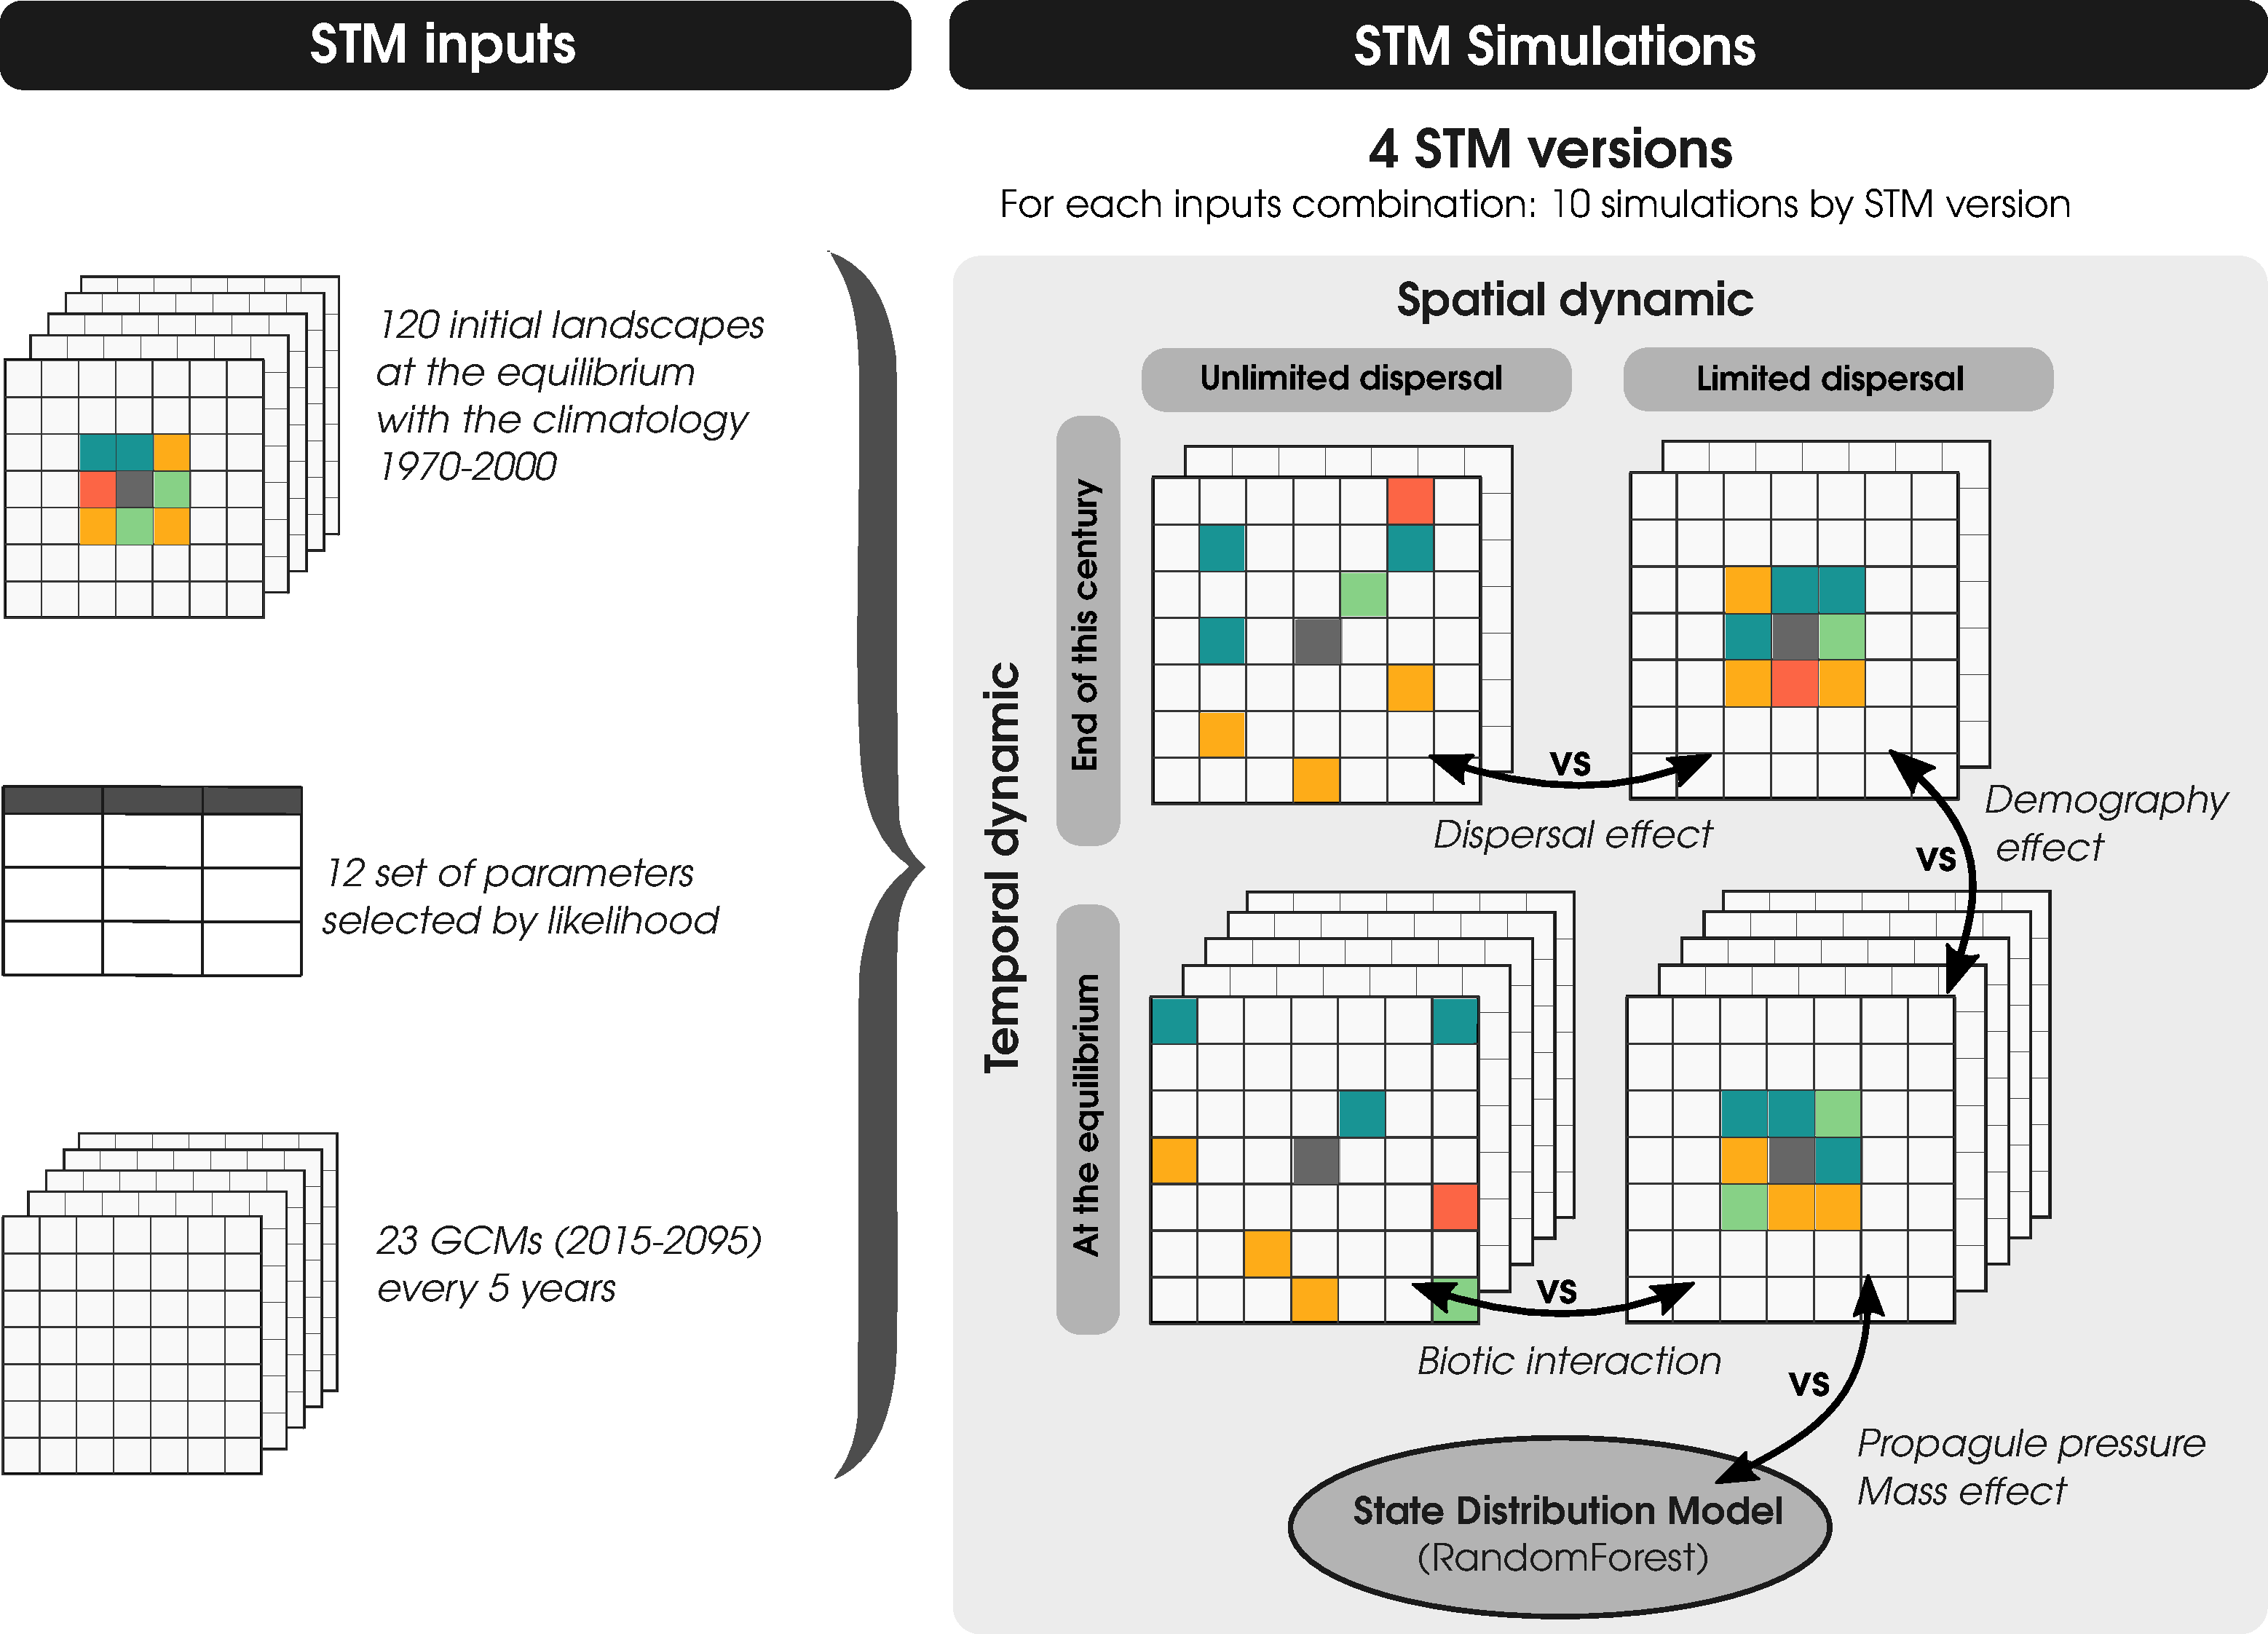
\includegraphics[width=0.8\textwidth]{figs/simus_redu_schema_v2.pdf}
	\end{center}
\end{figure}

% More justification
% Why we choose those climatic variable ? Those climatic variable have been recognized as a good combination to explain the distribution of the boreal forest \cite{Scheffer2012,Goldblum aussi}.

% Mise à l'échelle années pour les transitions


We incorporated three information types: (1) state transitions observed
between plot measurements, (2) the average climate of the 15 years before each
measurements for the two climatic variables of interest and finally the (3)
the proportion of states available in the neighbors using a SDM (RandomForest)
approach as a proxy.

% Ajouter une figure avec le workflow de la calibration

\subsection{Simulations and analysis}

1. How the model is implemented as spatial explicit ? Moore neighbors
Describe the initial simulation landscape and the choice of the resolution


We performed the simulations using 10 several initial landscape, and 12
different sets of parameters. For each parameters set and initial landscape,
we ran simulations over the climate predicted by the 23 Global Climate Models
(GCM) downscaled at 10 km$^2$ by the Ouranos consortium in clmatology in
Quebec. For each of those combinations, we replicated 10 times the simulation
in order to take in account the model stochasticty.

\section{Results}

A. Approximation of the neighbors (SDM)
Ajouter la stats du HK pour la validation croisé du modèle.

B. Model simulations

\begin{figure}
	\begin{center}
		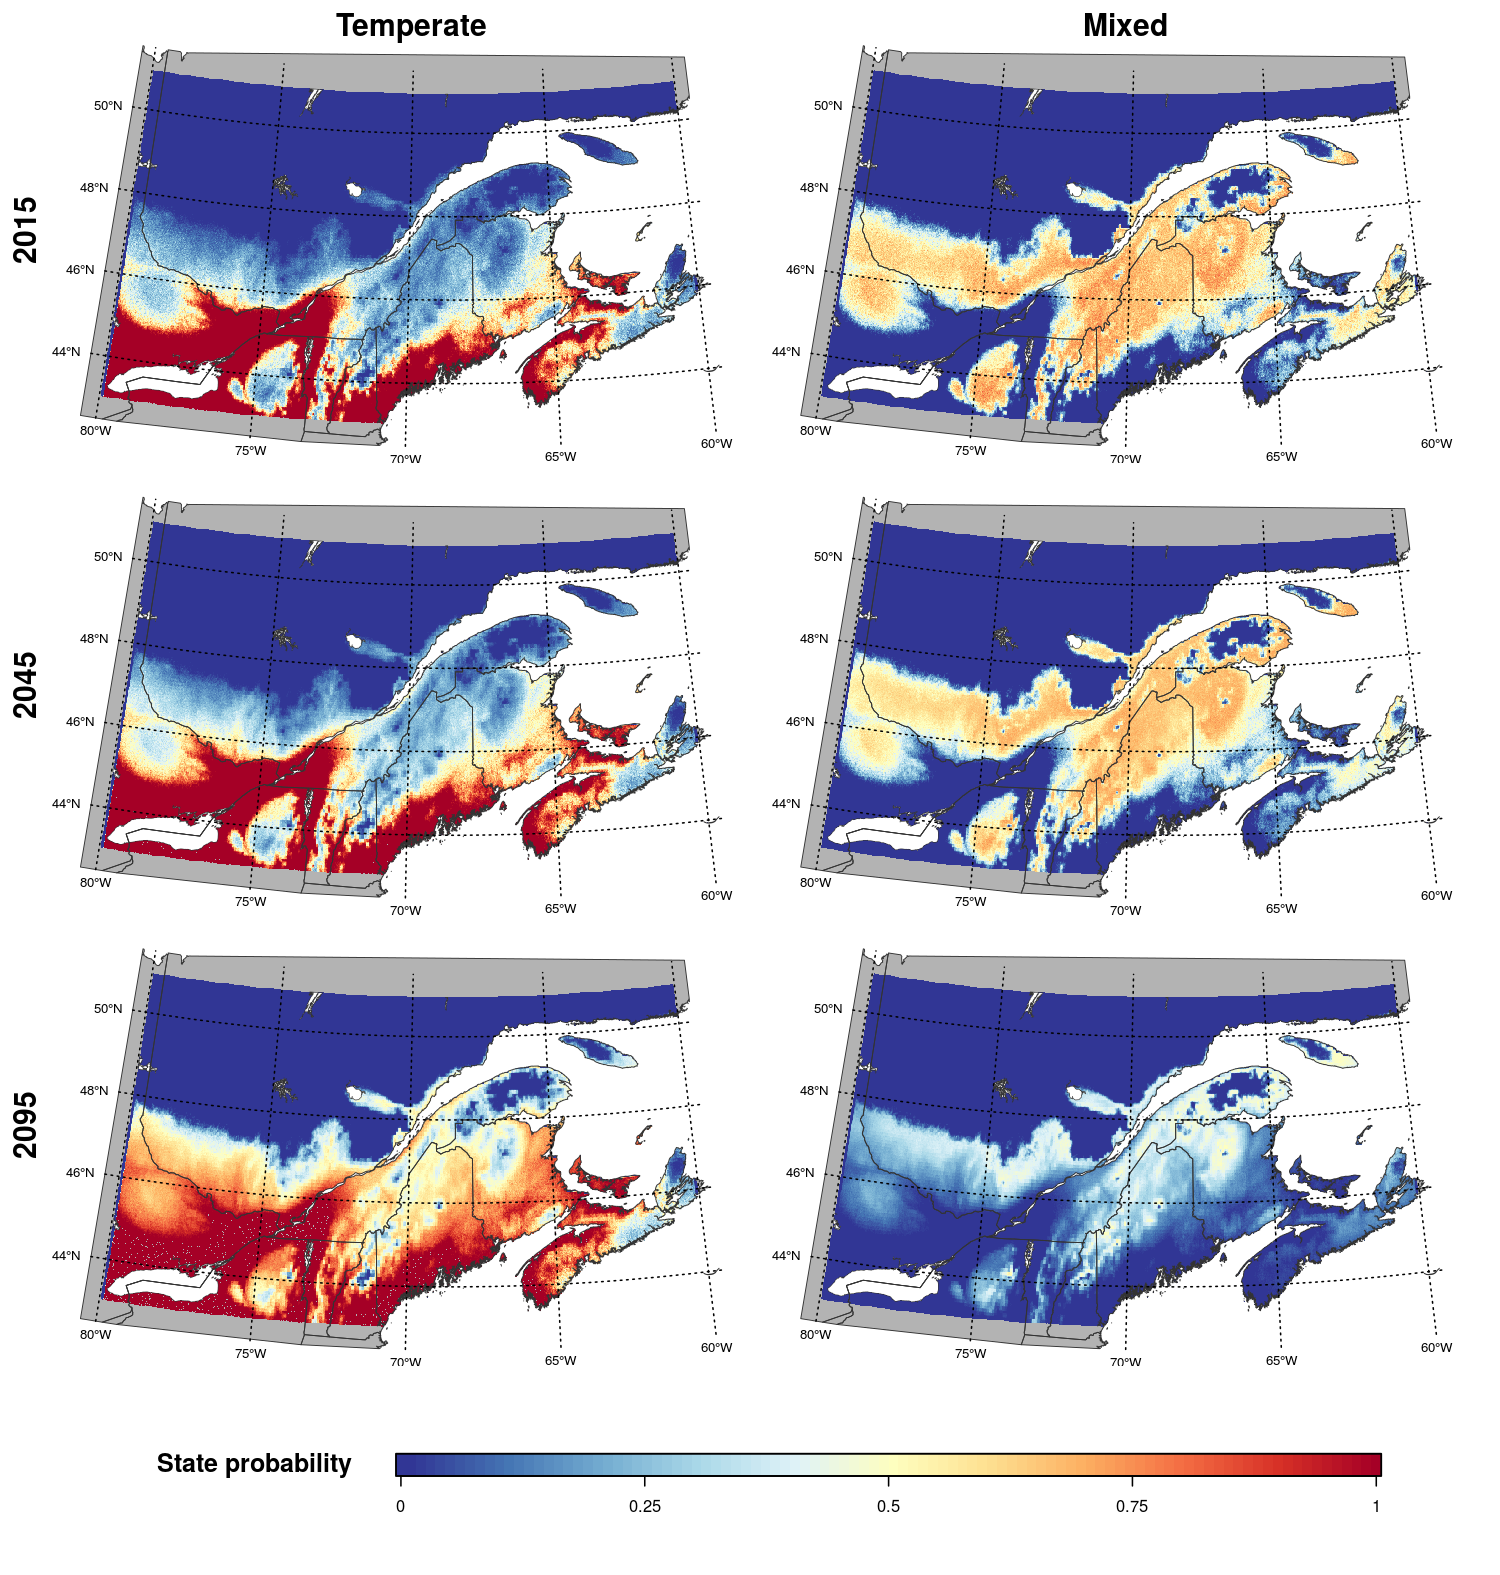
\includegraphics[width=\textwidth]{figs/future_distrib_states.png}
	\end{center}
\end{figure}

%Should I add an isocline representing the probability of 1 (predicted by the STM) to observe temperate forest?

Facultatif. We found that the STM was able to almost reproduce the actual distribution of the temperate forest and boreal forest.
1. Replacement of mixed forests by temperate forest
2. Long term simulations suggest a further but extremely slow colonization of the temperate forest northward

\begin{figure}
	\begin{center}
		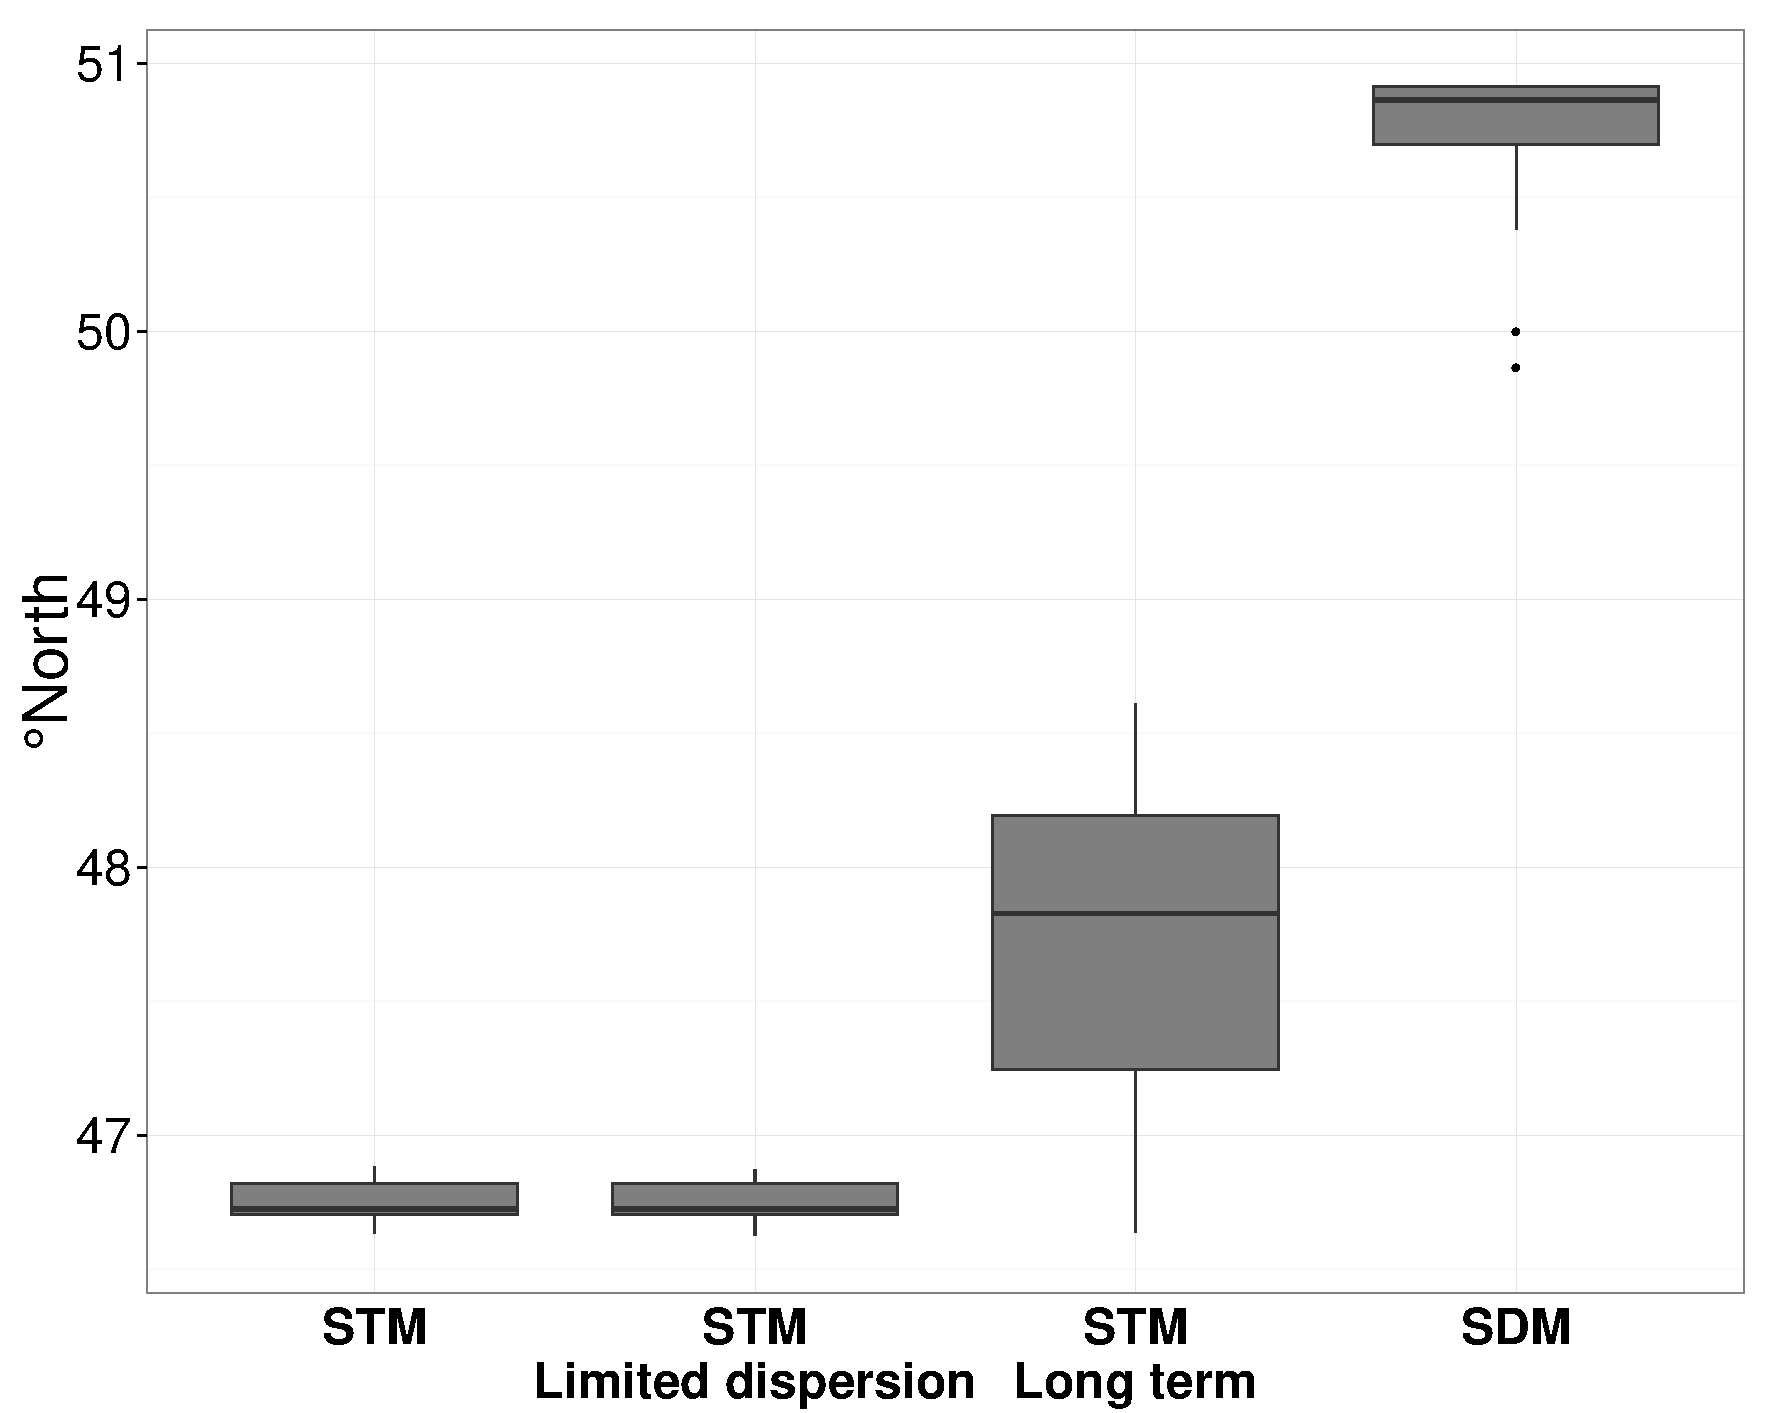
\includegraphics[width=0.5\textwidth]{figs/lat_max.pdf}
	\end{center}
\end{figure}

Slow temperate forest demography constrains migration rate more than dispersal limitation. Using the unlimited dispersion version, we predicted that the temperate forest

Spatial interaction prevents the temperate forest to fullfil its predicted niche (SDM) within an ecological timescale.

Complementary analysis on boxplot:
We identified that the STM version explains 90 \% of the latitudinal variance.

The model stochasticity (10 replicates)
The environnemental stochasicity (GCM's; n=23)
Parameters sensitivity (n=12)


New response curve: No leading edge but a higher abondances at the edge. This respond form is uncovered in the \cite{Lenoir2014a} article.


% TODO
%  Complément à apporter dans l'introduction et la conclusion. Importance de l'écologie forestièere vue par Cléments. L'approche par communauté forestière permet de simplifier le travail de conservation.


\clearpage
\bibliography{/home/steve/Dropbox/Bibtex/Master}

\end{document}
